% numerical.tex

\cleardoublepage
\chapter{Full Trajectory Optimisation}\label{chapter:numerical}

\textcolor{red}{add third stage, matrix and trajectory}



\begin{itemize}
	\item Details of bounds \& guesses, with reasoning. 
	\item Optimisation of the combined ascent and fly-back trajectories of the SPARTAN.
	\item Potential Abort Analysis
\end{itemize}


-sonic boom estimation?

-alternate trajectory recommendation?


\begin{figure}
	\centering
	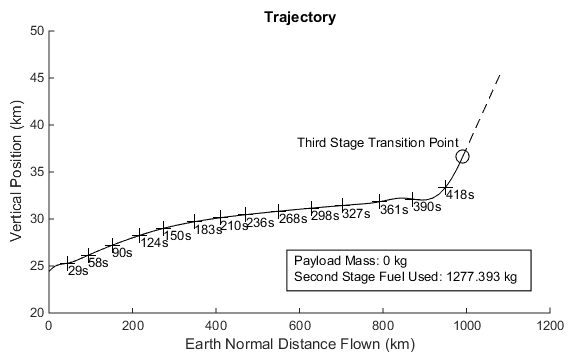
\includegraphics[width=0.9\linewidth]{figures/7_Full/Ascent}
	\caption{}
	\label{fig:ascent}
\end{figure}


\begin{figure}
	\centering
	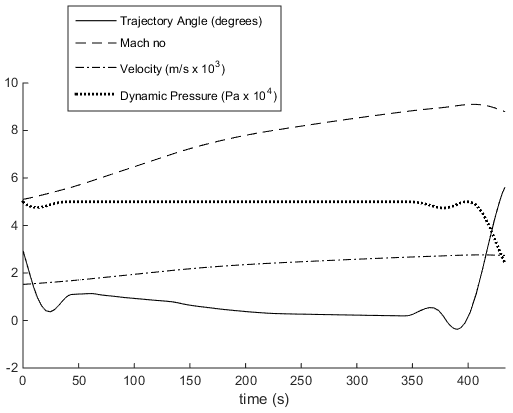
\includegraphics[width=0.7\linewidth]{figures/7_Full/Ascent-Aero}
	\caption{}
	\label{fig:ascent-aero}
\end{figure}
\begin{figure}
	\centering
	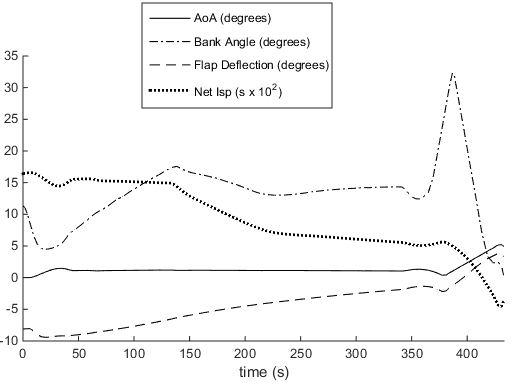
\includegraphics[width=0.7\linewidth]{figures/7_Full/Ascent-Vehicle}
	\caption{}
	\label{fig:ascent-vehicle}
\end{figure}


\begin{figure}
	\centering
	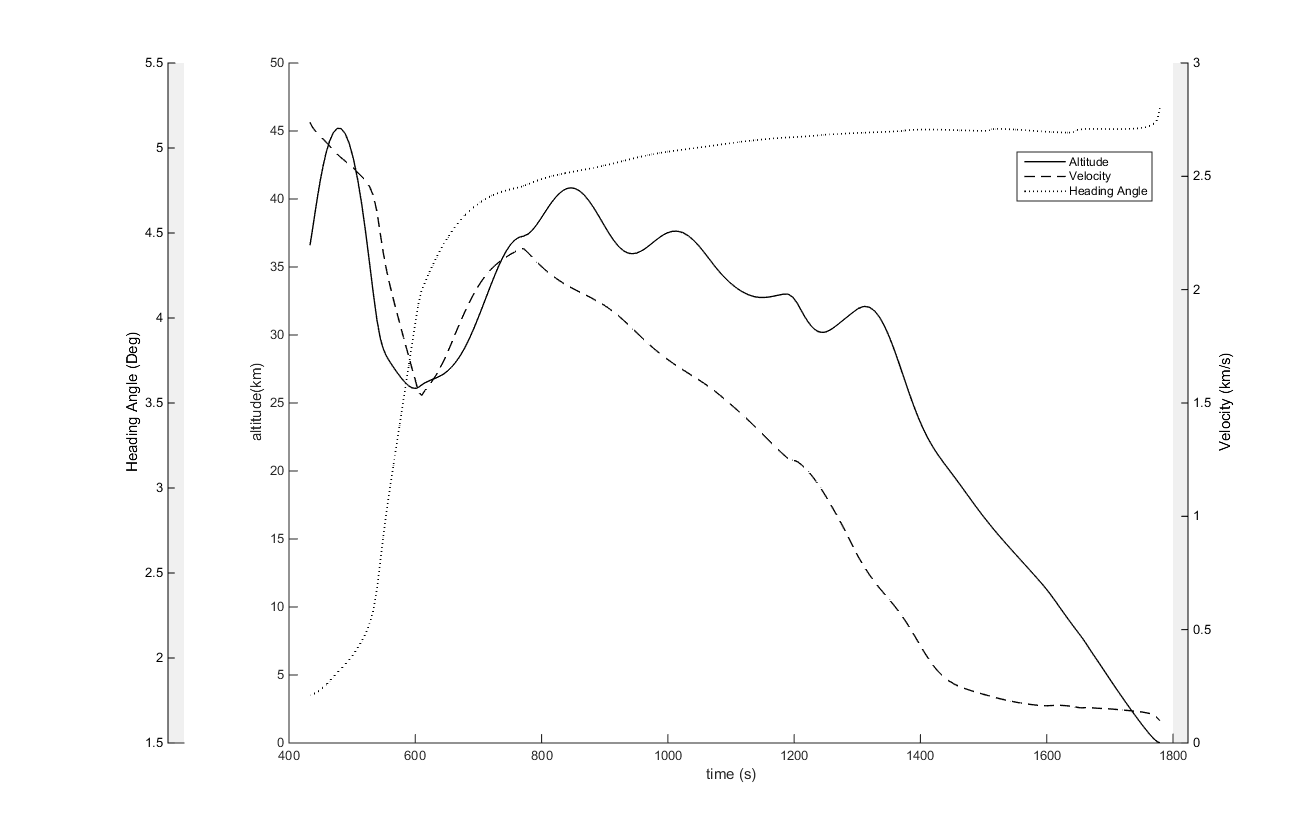
\includegraphics[width=0.7\linewidth]{figures/7_Full/FlyBack1}
	\caption{}
	\label{fig:flyback1}
\end{figure}






\begin{figure}
	\centering
	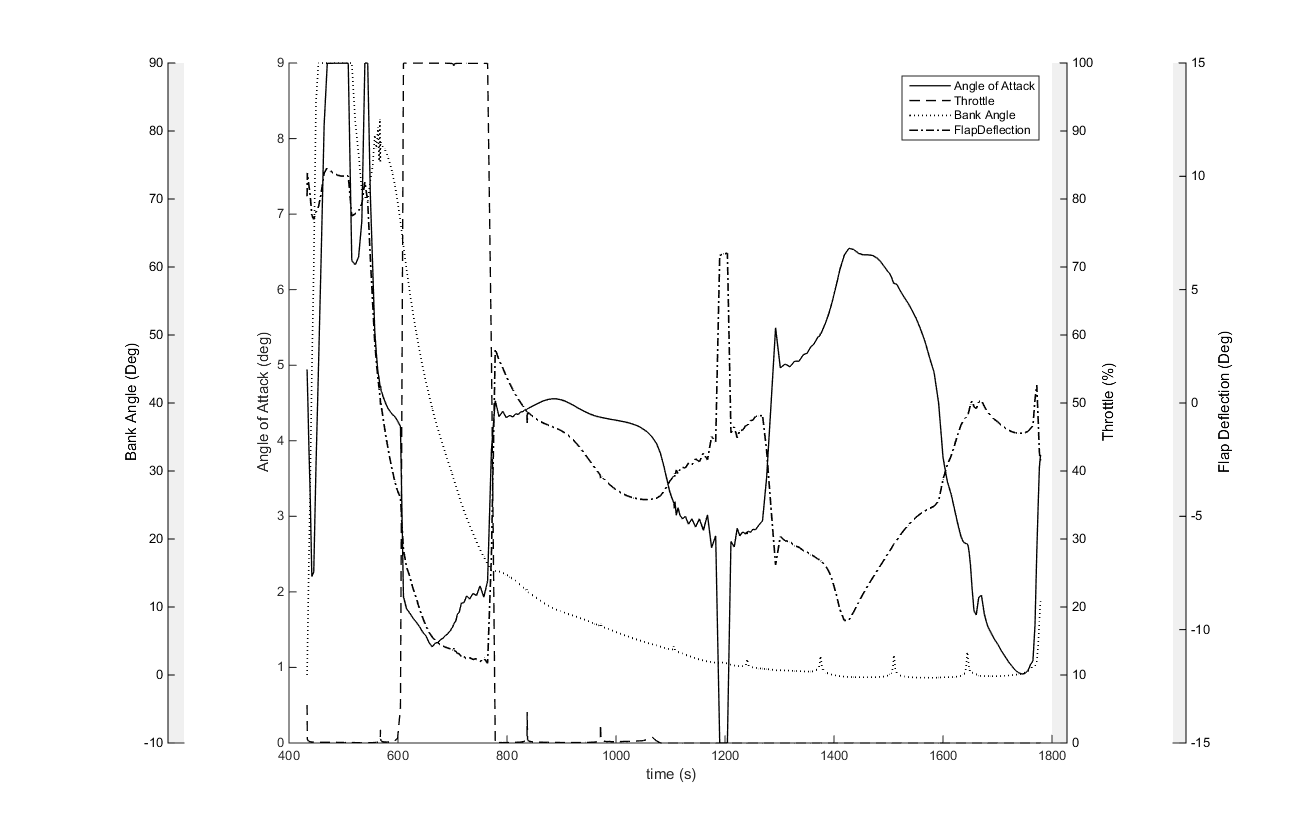
\includegraphics[width=0.7\linewidth]{figures/7_Full/FlyBack2}
	\caption{}
	\label{fig:flyback2}
\end{figure}


\begin{figure}
	\centering
	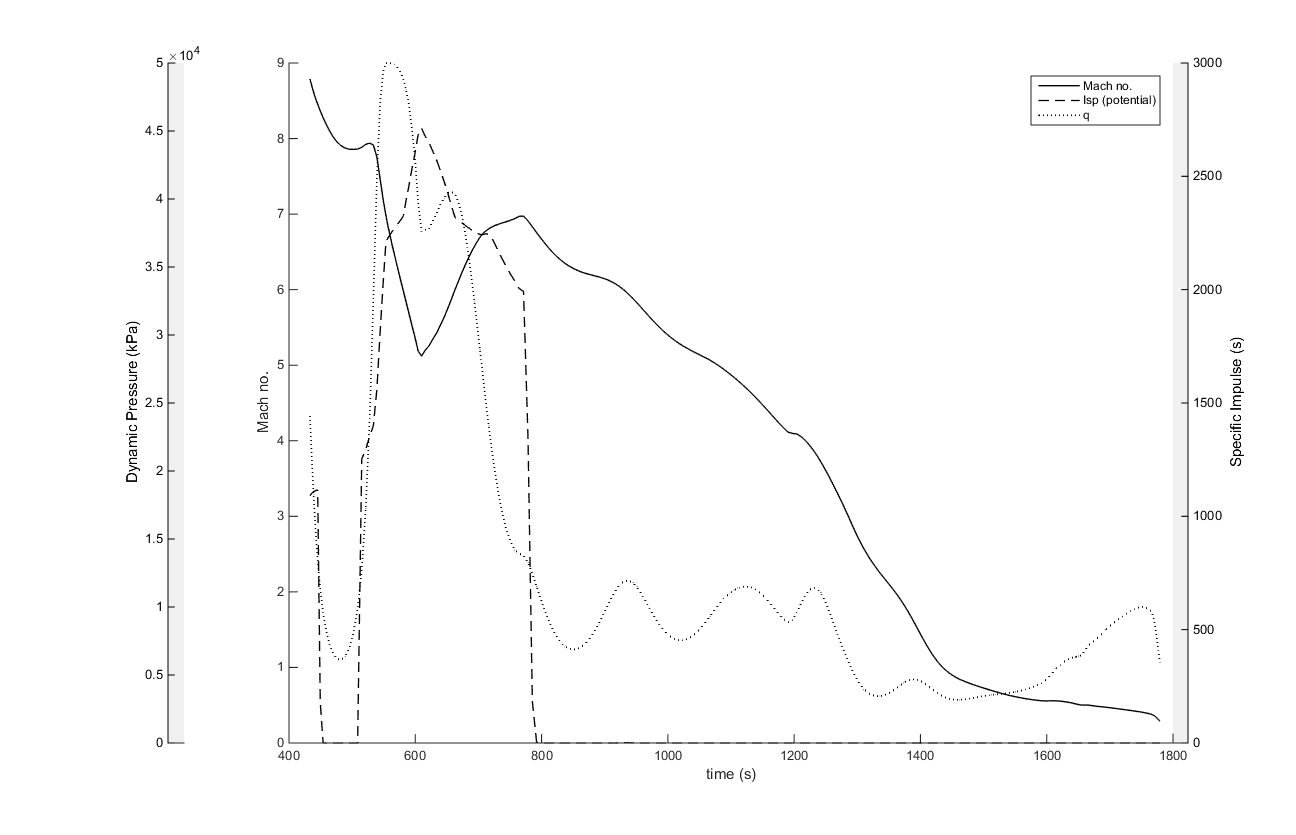
\includegraphics[width=0.7\linewidth]{figures/7_Full/FlyBack3}
	\caption{}
	\label{fig:flyback3}
\end{figure}

\begin{figure}
	\centering
	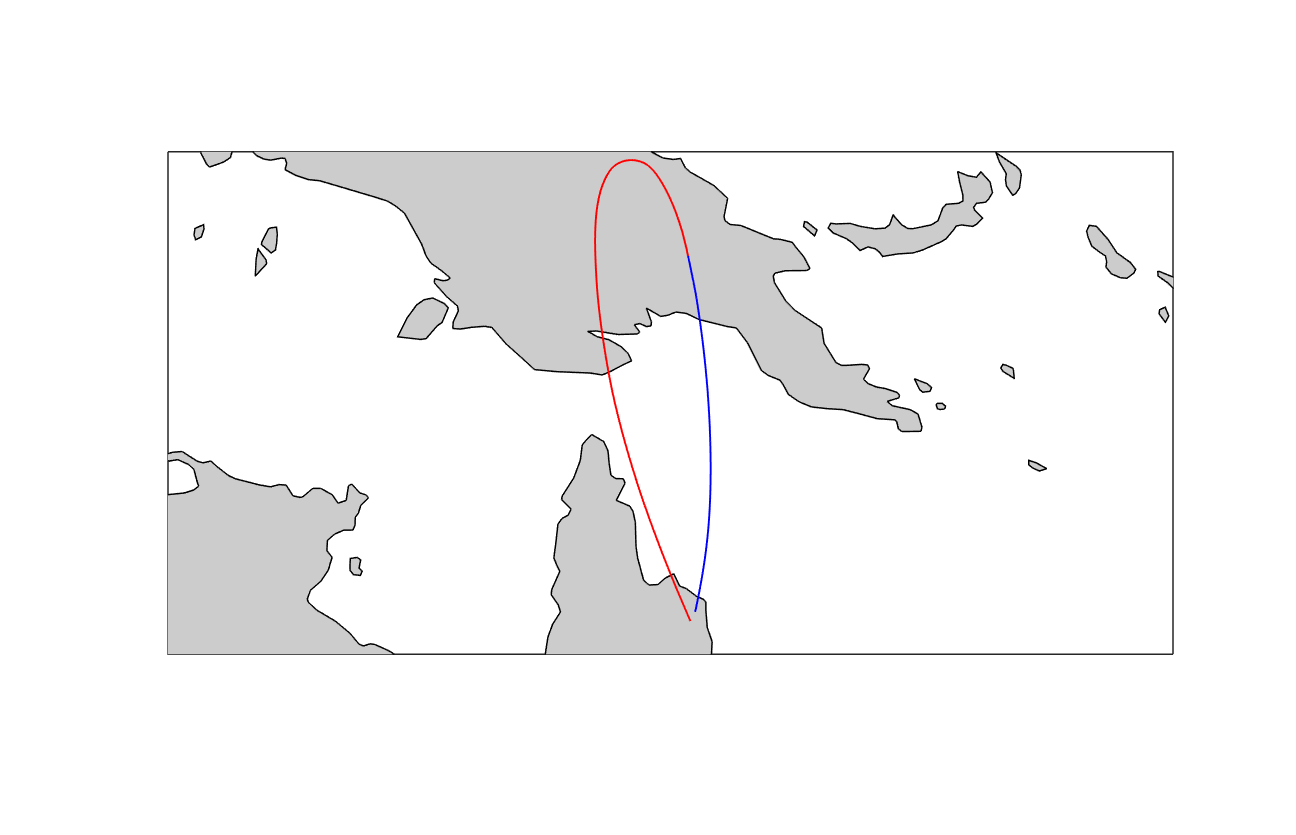
\includegraphics[width=0.7\linewidth]{figures/7_Full/groundtrack}
	\caption{}
	\label{fig:groundtrack}
\end{figure}


